\documentclass[1p]{elsarticle_modified}
%\bibliographystyle{elsarticle-num}

%\usepackage[colorlinks]{hyperref}
%\usepackage{abbrmath_seonhwa} %\Abb, \Ascr, \Acal ,\Abf, \Afrak
\usepackage{amsfonts}
\usepackage{amssymb}
\usepackage{amsmath}
\usepackage{amsthm}
\usepackage{scalefnt}
\usepackage{amsbsy}
\usepackage{kotex}
\usepackage{caption}
\usepackage{subfig}
\usepackage{color}
\usepackage{graphicx}
\usepackage{xcolor} %% white, black, red, green, blue, cyan, magenta, yellow
\usepackage{float}
\usepackage{setspace}
\usepackage{hyperref}

\usepackage{tikz}
\usetikzlibrary{arrows}

\usepackage{multirow}
\usepackage{array} % fixed length table
\usepackage{hhline}

%%%%%%%%%%%%%%%%%%%%%
\makeatletter
\renewcommand*\env@matrix[1][\arraystretch]{%
	\edef\arraystretch{#1}%
	\hskip -\arraycolsep
	\let\@ifnextchar\new@ifnextchar
	\array{*\c@MaxMatrixCols c}}
\makeatother %https://tex.stackexchange.com/questions/14071/how-can-i-increase-the-line-spacing-in-a-matrix
%%%%%%%%%%%%%%%

\usepackage[normalem]{ulem}

\newcommand{\msout}[1]{\ifmmode\text{\sout{\ensuremath{#1}}}\else\sout{#1}\fi}
%SOURCE: \msout is \stkout macro in https://tex.stackexchange.com/questions/20609/strikeout-in-math-mode

\newcommand{\cancel}[1]{
	\ifmmode
	{\color{red}\msout{#1}}
	\else
	{\color{red}\sout{#1}}
	\fi
}

\newcommand{\add}[1]{
	{\color{blue}\uwave{#1}}
}

\newcommand{\replace}[2]{
	\ifmmode
	{\color{red}\msout{#1}}{\color{blue}\uwave{#2}}
	\else
	{\color{red}\sout{#1}}{\color{blue}\uwave{#2}}
	\fi
}

\newcommand{\Sol}{\mathcal{S}} %segment
\newcommand{\D}{D} %diagram
\newcommand{\A}{\mathcal{A}} %arc


%%%%%%%%%%%%%%%%%%%%%%%%%%%%%5 test

\def\sl{\operatorname{\textup{SL}}(2,\Cbb)}
\def\psl{\operatorname{\textup{PSL}}(2,\Cbb)}
\def\quan{\mkern 1mu \triangleright \mkern 1mu}

\theoremstyle{definition}
\newtheorem{thm}{Theorem}[section]
\newtheorem{prop}[thm]{Proposition}
\newtheorem{lem}[thm]{Lemma}
\newtheorem{ques}[thm]{Question}
\newtheorem{cor}[thm]{Corollary}
\newtheorem{defn}[thm]{Definition}
\newtheorem{exam}[thm]{Example}
\newtheorem{rmk}[thm]{Remark}
\newtheorem{alg}[thm]{Algorithm}

\newcommand{\I}{\sqrt{-1}}
\begin{document}

%\begin{frontmatter}
%
%\title{Boundary parabolic representations of knots up to 8 crossings}
%
%%% Group authors per affiliation:
%\author{Yunhi Cho} 
%\address{Department of Mathematics, University of Seoul, Seoul, Korea}
%\ead{yhcho@uos.ac.kr}
%
%
%\author{Seonhwa Kim} %\fnref{s_kim}}
%\address{Center for Geometry and Physics, Institute for Basic Science, Pohang, 37673, Korea}
%\ead{ryeona17@ibs.re.kr}
%
%\author{Hyuk Kim}
%\address{Department of Mathematical Sciences, Seoul National University, Seoul 08826, Korea}
%\ead{hyukkim@snu.ac.kr}
%
%\author{Seokbeom Yoon}
%\address{Department of Mathematical Sciences, Seoul National University, Seoul, 08826,  Korea}
%\ead{sbyoon15@snu.ac.kr}
%
%\begin{abstract}
%We find all boundary parabolic representation of knots up to 8 crossings.
%
%\end{abstract}
%\begin{keyword}
%    \MSC[2010] 57M25 
%\end{keyword}
%
%\end{frontmatter}

%\linenumbers
%\tableofcontents
%
\newcommand\colored[1]{\textcolor{white}{\rule[-0.35ex]{0.8em}{1.4ex}}\kern-0.8em\color{red} #1}%
%\newcommand\colored[1]{\textcolor{white}{ #1}\kern-2.17ex	\textcolor{white}{ #1}\kern-1.81ex	\textcolor{white}{ #1}\kern-2.15ex\color{red}#1	}

{\Large $\underline{12n_{0527}~(K12n_{0527})}$}

\setlength{\tabcolsep}{10pt}
\renewcommand{\arraystretch}{1.6}
\vspace{1cm}\begin{tabular}{m{100pt}>{\centering\arraybackslash}m{274pt}}
\multirow{5}{120pt}{
	\centering
	\includegraphics[width=112pt]{../../../GIT/diagram.site/Diagrams/png/2616_12n_0527.png}\\
\ \ \ A knot diagram\footnotemark}&
\allowdisplaybreaks
\textbf{Linearized knot diagam} \\
\cline{2-2}
 &
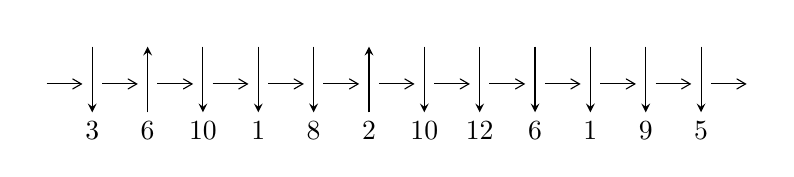
\begin{tikzpicture}[x=20pt, y=17pt]
	% nodes
	\node (C0) at (0, 0) {};
	\node (C1) at (1, 0) {};
	\node (C1U) at (1, +1) {};
	\node (C1D) at (1, -1) {3};

	\node (C2) at (2, 0) {};
	\node (C2U) at (2, +1) {};
	\node (C2D) at (2, -1) {6};

	\node (C3) at (3, 0) {};
	\node (C3U) at (3, +1) {};
	\node (C3D) at (3, -1) {10};

	\node (C4) at (4, 0) {};
	\node (C4U) at (4, +1) {};
	\node (C4D) at (4, -1) {1};

	\node (C5) at (5, 0) {};
	\node (C5U) at (5, +1) {};
	\node (C5D) at (5, -1) {8};

	\node (C6) at (6, 0) {};
	\node (C6U) at (6, +1) {};
	\node (C6D) at (6, -1) {2};

	\node (C7) at (7, 0) {};
	\node (C7U) at (7, +1) {};
	\node (C7D) at (7, -1) {10};

	\node (C8) at (8, 0) {};
	\node (C8U) at (8, +1) {};
	\node (C8D) at (8, -1) {12};

	\node (C9) at (9, 0) {};
	\node (C9U) at (9, +1) {};
	\node (C9D) at (9, -1) {6};

	\node (C10) at (10, 0) {};
	\node (C10U) at (10, +1) {};
	\node (C10D) at (10, -1) {1};

	\node (C11) at (11, 0) {};
	\node (C11U) at (11, +1) {};
	\node (C11D) at (11, -1) {9};

	\node (C12) at (12, 0) {};
	\node (C12U) at (12, +1) {};
	\node (C12D) at (12, -1) {5};
	\node (C13) at (13, 0) {};

	% arrows
	\draw[->,>={angle 60}]
	(C0) edge (C1) (C1) edge (C2) (C2) edge (C3) (C3) edge (C4) (C4) edge (C5) (C5) edge (C6) (C6) edge (C7) (C7) edge (C8) (C8) edge (C9) (C9) edge (C10) (C10) edge (C11) (C11) edge (C12) (C12) edge (C13) ;	\draw[->,>=stealth]
	(C1U) edge (C1D) (C2D) edge (C2U) (C3U) edge (C3D) (C4U) edge (C4D) (C5U) edge (C5D) (C6D) edge (C6U) (C7U) edge (C7D) (C8U) edge (C8D) (C9U) edge (C9D) (C10U) edge (C10D) (C11U) edge (C11D) (C12U) edge (C12D) ;
	\end{tikzpicture} \\
\hhline{~~} \\& 
\textbf{Solving Sequence} \\ \cline{2-2} 
 &
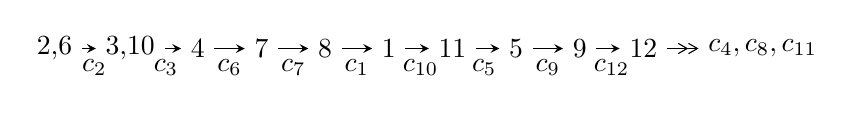
\begin{tikzpicture}[x=23pt, y=7pt]
	% node
	\node (A0) at (-1/8, 0) {2,6};
	\node (A1) at (17/16, 0) {3,10};
	\node (A2) at (17/8, 0) {4};
	\node (A3) at (25/8, 0) {7};
	\node (A4) at (33/8, 0) {8};
	\node (A5) at (41/8, 0) {1};
	\node (A6) at (49/8, 0) {11};
	\node (A7) at (57/8, 0) {5};
	\node (A8) at (65/8, 0) {9};
	\node (A9) at (73/8, 0) {12};
	\node (C1) at (1/2, -1) {$c_{2}$};
	\node (C2) at (13/8, -1) {$c_{3}$};
	\node (C3) at (21/8, -1) {$c_{6}$};
	\node (C4) at (29/8, -1) {$c_{7}$};
	\node (C5) at (37/8, -1) {$c_{1}$};
	\node (C6) at (45/8, -1) {$c_{10}$};
	\node (C7) at (53/8, -1) {$c_{5}$};
	\node (C8) at (61/8, -1) {$c_{9}$};
	\node (C9) at (69/8, -1) {$c_{12}$};
	\node (A10) at (11, 0) {$c_{4},c_{8},c_{11}$};

	% edge
	\draw[->,>=stealth]	
	(A0) edge (A1) (A1) edge (A2) (A2) edge (A3) (A3) edge (A4) (A4) edge (A5) (A5) edge (A6) (A6) edge (A7) (A7) edge (A8) (A8) edge (A9) ;
	\draw[->>,>={angle 60}]	
	(A9) edge (A10);
\end{tikzpicture} \\ 

\end{tabular} \\

\footnotetext{
The image of knot diagram is generated by the software ``\textbf{Draw programme}" developed by Andrew Bartholomew(\url{http://www.layer8.co.uk/maths/draw/index.htm\#Running-draw}), where we modified some parts for our purpose(\url{https://github.com/CATsTAILs/LinksPainter}).
}\phantom \\ \newline 
\centering \textbf{Ideals for irreducible components\footnotemark of $X_{\text{par}}$} 
 
\begin{align*}
I^u_{1}&=\langle 
378975 u^{30}+3018590 u^{29}+\cdots+228821 b-6857553,\\
\phantom{I^u_{1}}&\phantom{= \langle  }12363803 u^{30}+93404174 u^{29}+\cdots+2288210 a-220745786,\;u^{31}+8 u^{30}+\cdots-62 u-10\rangle \\
I^u_{2}&=\langle 
3 u^{18}-6 u^{17}+\cdots+2 b+2,\;-2 u^{18} a+10 u^{18}+\cdots-3 a+21,\;u^{19}-3 u^{18}+\cdots+6 u-1\rangle \\
I^u_{3}&=\langle 
u^{14}-4 u^{13}+12 u^{12}-24 u^{11}+40 u^{10}-52 u^9+57 u^8-49 u^7+34 u^6-18 u^5+6 u^4-2 u^3+b- u-1,\\
\phantom{I^u_{3}}&\phantom{= \langle  }u^{14}-3 u^{13}+7 u^{12}-8 u^{11}+4 u^{10}+12 u^9-34 u^8+58 u^7-68 u^6+62 u^5-44 u^4+24 u^3-11 u^2+2 a+5 u-4,\\
\phantom{I^u_{3}}&\phantom{= \langle  }u^{15}-5 u^{14}+\cdots+4 u-2\rangle \\
I^u_{4}&=\langle 
a^3 u- a^3+a^2 u- a^2+3 a u+3 b+u-1,\;a^4-3 a^2 u- a^2+2 a u+2 a-2 u-2,\;u^2+u+1\rangle \\
\\
\end{align*}
\raggedright * 4 irreducible components of $\dim_{\mathbb{C}}=0$, with total 92 representations.\\
\footnotetext{All coefficients of polynomials are rational numbers. But the coefficients are sometimes approximated in decimal forms when there is not enough margin.}
\newpage
\renewcommand{\arraystretch}{1}
\centering \section*{I. $I^u_{1}= \langle 3.79\times10^{5} u^{30}+3.02\times10^{6} u^{29}+\cdots+2.29\times10^{5} b-6.86\times10^{6},\;1.24\times10^{7} u^{30}+9.34\times10^{7} u^{29}+\cdots+2.29\times10^{6} a-2.21\times10^{8},\;u^{31}+8 u^{30}+\cdots-62 u-10 \rangle$}
\flushleft \textbf{(i) Arc colorings}\\
\begin{tabular}{m{7pt} m{180pt} m{7pt} m{180pt} }
\flushright $a_{2}=$&$\begin{pmatrix}1\\0\end{pmatrix}$ \\
\flushright $a_{6}=$&$\begin{pmatrix}0\\u\end{pmatrix}$ \\
\flushright $a_{3}=$&$\begin{pmatrix}1\\- u^2\end{pmatrix}$ \\
\flushright $a_{10}=$&$\begin{pmatrix}-5.40326 u^{30}-40.8198 u^{29}+\cdots+422.621 u+96.4709\\-1.65621 u^{30}-13.1919 u^{29}+\cdots+143.370 u+29.9691\end{pmatrix}$ \\
\flushright $a_{4}=$&$\begin{pmatrix}-7.59786 u^{30}-57.1445 u^{29}+\cdots+582.083 u+133.417\\-2.53663 u^{30}-19.5572 u^{29}+\cdots+189.049 u+39.5947\end{pmatrix}$ \\
\flushright $a_{7}=$&$\begin{pmatrix}u\\u\end{pmatrix}$ \\
\flushright $a_{8}=$&$\begin{pmatrix}-5.06123 u^{30}-37.5873 u^{29}+\cdots+394.034 u+92.8223\\-1.48595 u^{30}-10.9890 u^{29}+\cdots+92.6272 u+21.5867\end{pmatrix}$ \\
\flushright $a_{1}=$&$\begin{pmatrix}u^2+1\\- u^4\end{pmatrix}$ \\
\flushright $a_{11}=$&$\begin{pmatrix}-2.01783 u^{30}-15.2733 u^{29}+\cdots+183.285 u+43.3542\\-0.349286 u^{30}-3.00908 u^{29}+\cdots+131.287 u+29.6924\end{pmatrix}$ \\
\flushright $a_{5}=$&$\begin{pmatrix}-4.17727 u^{30}-31.3609 u^{29}+\cdots+302.304 u+68.6386\\-2.36578 u^{30}-18.6263 u^{29}+\cdots+194.064 u+41.2391\end{pmatrix}$ \\
\flushright $a_{9}=$&$\begin{pmatrix}-5.40326 u^{30}-40.8198 u^{29}+\cdots+422.621 u+96.4709\\-0.906058 u^{30}-7.88315 u^{29}+\cdots+48.2085 u+5.90550\end{pmatrix}$ \\
\flushright $a_{12}=$&$\begin{pmatrix}2.85487 u^{30}+20.6866 u^{29}+\cdots-172.102 u-39.1897\\-0.816394 u^{30}-6.48291 u^{29}+\cdots+188.974 u+41.4018\end{pmatrix}$\\&\end{tabular}
\flushleft \textbf{(ii) Obstruction class $= -1$}\\~\\
\flushleft \textbf{(iii) Cusp Shapes $= -\frac{1324375}{228821} u^{30}-\frac{9572041}{228821} u^{29}+\cdots+\frac{117530906}{228821} u+\frac{30556088}{228821}$}\\~\\
\newpage\renewcommand{\arraystretch}{1}
\flushleft \textbf{(iv) u-Polynomials at the component}\newline \\
\begin{tabular}{m{50pt}|m{274pt}}
Crossings & \hspace{64pt}u-Polynomials at each crossing \\
\hline $$\begin{aligned}c_{1}\end{aligned}$$&$\begin{aligned}
&u^{31}+20 u^{30}+\cdots+684 u-100
\end{aligned}$\\
\hline $$\begin{aligned}c_{2},c_{6}\end{aligned}$$&$\begin{aligned}
&u^{31}-8 u^{30}+\cdots-62 u+10
\end{aligned}$\\
\hline $$\begin{aligned}c_{3},c_{9}\end{aligned}$$&$\begin{aligned}
&u^{31}+u^{30}+\cdots+u+1
\end{aligned}$\\
\hline $$\begin{aligned}c_{4},c_{5},c_{12}\end{aligned}$$&$\begin{aligned}
&u^{31}- u^{30}+\cdots+4 u+1
\end{aligned}$\\
\hline $$\begin{aligned}c_{7},c_{10}\end{aligned}$$&$\begin{aligned}
&u^{31}-3 u^{30}+\cdots+5 u+1
\end{aligned}$\\
\hline $$\begin{aligned}c_{8},c_{11}\end{aligned}$$&$\begin{aligned}
&u^{31}-11 u^{30}+\cdots-122 u+10
\end{aligned}$\\
\hline
\end{tabular}\\~\\
\newpage\renewcommand{\arraystretch}{1}
\flushleft \textbf{(v) Riley Polynomials at the component}\newline \\
\begin{tabular}{m{50pt}|m{274pt}}
Crossings & \hspace{64pt}Riley Polynomials at each crossing \\
\hline $$\begin{aligned}c_{1}\end{aligned}$$&$\begin{aligned}
&y^{31}-12 y^{30}+\cdots+1252656 y-10000
\end{aligned}$\\
\hline $$\begin{aligned}c_{2},c_{6}\end{aligned}$$&$\begin{aligned}
&y^{31}+20 y^{30}+\cdots+684 y-100
\end{aligned}$\\
\hline $$\begin{aligned}c_{3},c_{9}\end{aligned}$$&$\begin{aligned}
&y^{31}-29 y^{30}+\cdots+23 y-1
\end{aligned}$\\
\hline $$\begin{aligned}c_{4},c_{5},c_{12}\end{aligned}$$&$\begin{aligned}
&y^{31}+25 y^{30}+\cdots-6 y-1
\end{aligned}$\\
\hline $$\begin{aligned}c_{7},c_{10}\end{aligned}$$&$\begin{aligned}
&y^{31}-29 y^{30}+\cdots-105 y-1
\end{aligned}$\\
\hline $$\begin{aligned}c_{8},c_{11}\end{aligned}$$&$\begin{aligned}
&y^{31}+11 y^{30}+\cdots-756 y-100
\end{aligned}$\\
\hline
\end{tabular}\\~\\
\newpage\flushleft \textbf{(vi) Complex Volumes and Cusp Shapes}
$$\begin{array}{c|c|c}  
\text{Solutions to }I^u_{1}& \I (\text{vol} + \sqrt{-1}CS) & \text{Cusp shape}\\
 \hline 
\begin{aligned}
u &= -0.443501 + 0.881894 I \\
a &= -1.036980 - 0.315517 I \\
b &= -1.093880 - 0.219923 I\end{aligned}
 & \phantom{-}1.62568 - 2.07908 I & -8.15071 + 3.76851 I \\ \hline\begin{aligned}
u &= -0.443501 - 0.881894 I \\
a &= -1.036980 + 0.315517 I \\
b &= -1.093880 + 0.219923 I\end{aligned}
 & \phantom{-}1.62568 + 2.07908 I & -8.15071 - 3.76851 I \\ \hline\begin{aligned}
u &= -0.123465 + 0.920678 I \\
a &= -0.63652 + 1.53942 I \\
b &= \phantom{-}0.45891 + 1.91281 I\end{aligned}
 & \phantom{-}2.16097 - 0.39271 I & -5.96156 - 1.22021 I \\ \hline\begin{aligned}
u &= -0.123465 - 0.920678 I \\
a &= -0.63652 - 1.53942 I \\
b &= \phantom{-}0.45891 - 1.91281 I\end{aligned}
 & \phantom{-}2.16097 + 0.39271 I & -5.96156 + 1.22021 I \\ \hline\begin{aligned}
u &= \phantom{-}0.068946 + 1.101890 I \\
a &= \phantom{-}0.291434 - 0.967985 I \\
b &= -0.88132 - 1.46936 I\end{aligned}
 & \phantom{-}0.870446 + 0.149756 I & -6.74421 + 0.11134 I \\ \hline\begin{aligned}
u &= \phantom{-}0.068946 - 1.101890 I \\
a &= \phantom{-}0.291434 + 0.967985 I \\
b &= -0.88132 + 1.46936 I\end{aligned}
 & \phantom{-}0.870446 - 0.149756 I & -6.74421 - 0.11134 I \\ \hline\begin{aligned}
u &= -1.104440 + 0.109617 I \\
a &= -1.138250 - 0.420860 I \\
b &= \phantom{-}0.173388 - 0.107344 I\end{aligned}
 & -4.10069 - 3.26217 I & -7.80399 + 3.14222 I \\ \hline\begin{aligned}
u &= -1.104440 - 0.109617 I \\
a &= -1.138250 + 0.420860 I \\
b &= \phantom{-}0.173388 + 0.107344 I\end{aligned}
 & -4.10069 + 3.26217 I & -7.80399 - 3.14222 I \\ \hline\begin{aligned}
u &= -1.120450 + 0.048451 I \\
a &= \phantom{-}1.313720 - 0.318482 I \\
b &= -0.155061 + 0.121217 I\end{aligned}
 & -1.92223 + 10.09630 I & -6.60164 - 5.79982 I \\ \hline\begin{aligned}
u &= -1.120450 - 0.048451 I \\
a &= \phantom{-}1.313720 + 0.318482 I \\
b &= -0.155061 - 0.121217 I\end{aligned}
 & -1.92223 - 10.09630 I & -6.60164 + 5.79982 I\\
 \hline 
 \end{array}$$\newpage$$\begin{array}{c|c|c}  
\text{Solutions to }I^u_{1}& \I (\text{vol} + \sqrt{-1}CS) & \text{Cusp shape}\\
 \hline 
\begin{aligned}
u &= \phantom{-}0.805043 + 0.864131 I \\
a &= \phantom{-}0.256473 + 0.055333 I \\
b &= -0.056375 - 0.617551 I\end{aligned}
 & \phantom{-}6.77889 + 0.72800 I & \phantom{-}1.42894 - 3.61029 I \\ \hline\begin{aligned}
u &= \phantom{-}0.805043 - 0.864131 I \\
a &= \phantom{-}0.256473 - 0.055333 I \\
b &= -0.056375 + 0.617551 I\end{aligned}
 & \phantom{-}6.77889 - 0.72800 I & \phantom{-}1.42894 + 3.61029 I \\ \hline\begin{aligned}
u &= \phantom{-}0.106357 + 1.194790 I \\
a &= -0.585604 + 0.611175 I \\
b &= \phantom{-}0.11850 + 1.64905 I\end{aligned}
 & -4.49263 + 1.56261 I & -18.4490 - 2.4112 I \\ \hline\begin{aligned}
u &= \phantom{-}0.106357 - 1.194790 I \\
a &= -0.585604 - 0.611175 I \\
b &= \phantom{-}0.11850 - 1.64905 I\end{aligned}
 & -4.49263 - 1.56261 I & -18.4490 + 2.4112 I \\ \hline\begin{aligned}
u &= -0.255201 + 0.720413 I \\
a &= \phantom{-}0.353004 - 0.498369 I \\
b &= \phantom{-}0.074523 - 0.477887 I\end{aligned}
 & -0.379147 - 1.186170 I & -4.44708 + 5.86244 I \\ \hline\begin{aligned}
u &= -0.255201 - 0.720413 I \\
a &= \phantom{-}0.353004 + 0.498369 I \\
b &= \phantom{-}0.074523 + 0.477887 I\end{aligned}
 & -0.379147 + 1.186170 I & -4.44708 - 5.86244 I \\ \hline\begin{aligned}
u &= -0.287076 + 1.208000 I \\
a &= \phantom{-}0.591625 - 1.023160 I \\
b &= \phantom{-}0.45808 - 2.00681 I\end{aligned}
 & -0.11428 - 4.16519 I & -8.00000 + 3.45619 I \\ \hline\begin{aligned}
u &= -0.287076 - 1.208000 I \\
a &= \phantom{-}0.591625 + 1.023160 I \\
b &= \phantom{-}0.45808 + 2.00681 I\end{aligned}
 & -0.11428 + 4.16519 I & -8.00000 - 3.45619 I \\ \hline\begin{aligned}
u &= \phantom{-}0.839144 + 0.959645 I \\
a &= -0.126368 + 0.182032 I \\
b &= \phantom{-}0.546509 + 0.211498 I\end{aligned}
 & \phantom{-}6.52389 + 5.44822 I & -3.50283 + 0. I\phantom{ +0.000000I} \\ \hline\begin{aligned}
u &= \phantom{-}0.839144 - 0.959645 I \\
a &= -0.126368 - 0.182032 I \\
b &= \phantom{-}0.546509 - 0.211498 I\end{aligned}
 & \phantom{-}6.52389 - 5.44822 I & -3.50283 + 0. I\phantom{ +0.000000I}\\
 \hline 
 \end{array}$$\newpage$$\begin{array}{c|c|c}  
\text{Solutions to }I^u_{1}& \I (\text{vol} + \sqrt{-1}CS) & \text{Cusp shape}\\
 \hline 
\begin{aligned}
u &= -0.55841 + 1.36375 I \\
a &= -0.031464 - 1.250450 I \\
b &= \phantom{-}0.13295 - 2.63897 I\end{aligned}
 & -6.0602 - 16.0464 I & \phantom{-0.000000 } 0 \\ \hline\begin{aligned}
u &= -0.55841 - 1.36375 I \\
a &= -0.031464 + 1.250450 I \\
b &= \phantom{-}0.13295 + 2.63897 I\end{aligned}
 & -6.0602 + 16.0464 I & \phantom{-0.000000 } 0 \\ \hline\begin{aligned}
u &= -0.523642 + 0.015251 I \\
a &= \phantom{-}1.36675 + 1.50756 I \\
b &= \phantom{-}0.340155 + 0.377383 I\end{aligned}
 & \phantom{-}3.48762 - 1.00607 I & -1.97801 + 2.70347 I \\ \hline\begin{aligned}
u &= -0.523642 - 0.015251 I \\
a &= \phantom{-}1.36675 - 1.50756 I \\
b &= \phantom{-}0.340155 - 0.377383 I\end{aligned}
 & \phantom{-}3.48762 + 1.00607 I & -1.97801 - 2.70347 I \\ \hline\begin{aligned}
u &= -0.47698 + 1.40113 I \\
a &= -0.090020 + 1.114860 I \\
b &= -0.12726 + 2.47258 I\end{aligned}
 & -8.91065 - 8.81717 I & \phantom{-0.000000 } 0 \\ \hline\begin{aligned}
u &= -0.47698 - 1.40113 I \\
a &= -0.090020 - 1.114860 I \\
b &= -0.12726 - 2.47258 I\end{aligned}
 & -8.91065 + 8.81717 I & \phantom{-0.000000 } 0 \\ \hline\begin{aligned}
u &= -0.59892 + 1.37175 I \\
a &= \phantom{-}0.349486 + 0.852345 I \\
b &= \phantom{-}0.51025 + 1.90344 I\end{aligned}
 & -8.00712 - 2.87739 I & \phantom{-0.000000 } 0 \\ \hline\begin{aligned}
u &= -0.59892 - 1.37175 I \\
a &= \phantom{-}0.349486 - 0.852345 I \\
b &= \phantom{-}0.51025 - 1.90344 I\end{aligned}
 & -8.00712 + 2.87739 I & \phantom{-0.000000 } 0 \\ \hline\begin{aligned}
u &= -0.48869 + 1.42613 I \\
a &= -0.291444 - 0.902646 I \\
b &= -0.69470 - 2.05198 I\end{aligned}
 & -6.65609 + 4.30866 I & \phantom{-0.000000 } 0 \\ \hline\begin{aligned}
u &= -0.48869 - 1.42613 I \\
a &= -0.291444 + 0.902646 I \\
b &= -0.69470 + 2.05198 I\end{aligned}
 & -6.65609 - 4.30866 I & \phantom{-0.000000 } 0\\
 \hline 
 \end{array}$$\newpage$$\begin{array}{c|c|c}  
\text{Solutions to }I^u_{1}& \I (\text{vol} + \sqrt{-1}CS) & \text{Cusp shape}\\
 \hline 
\begin{aligned}
u &= \phantom{-}0.322569\phantom{ +0.000000I} \\
a &= \phantom{-}1.42830\phantom{ +0.000000I} \\
b &= -0.609341\phantom{ +0.000000I}\end{aligned}
 & -1.08738\phantom{ +0.000000I} & -6.65470\phantom{ +0.000000I}\\
 \hline 
 \end{array}$$\newpage\newpage\renewcommand{\arraystretch}{1}
\centering \section*{II. $I^u_{2}= \langle 3 u^{18}-6 u^{17}+\cdots+2 b+2,\;-2 u^{18} a+10 u^{18}+\cdots-3 a+21,\;u^{19}-3 u^{18}+\cdots+6 u-1 \rangle$}
\flushleft \textbf{(i) Arc colorings}\\
\begin{tabular}{m{7pt} m{180pt} m{7pt} m{180pt} }
\flushright $a_{2}=$&$\begin{pmatrix}1\\0\end{pmatrix}$ \\
\flushright $a_{6}=$&$\begin{pmatrix}0\\u\end{pmatrix}$ \\
\flushright $a_{3}=$&$\begin{pmatrix}1\\- u^2\end{pmatrix}$ \\
\flushright $a_{10}=$&$\begin{pmatrix}a\\-\frac{3}{2} u^{18}+3 u^{17}+\cdots+\frac{9}{2} u-1\end{pmatrix}$ \\
\flushright $a_{4}=$&$\begin{pmatrix}-\frac{3}{2} u^{18}+4 u^{17}+\cdots+\frac{39}{2} u-4\\-\frac{3}{2} u^{18} a-\frac{1}{2} u^{18}+\cdots-\frac{3}{2} a+3\end{pmatrix}$ \\
\flushright $a_{7}=$&$\begin{pmatrix}u\\u\end{pmatrix}$ \\
\flushright $a_{8}=$&$\begin{pmatrix}-\frac{3}{2} u^{18} a+u^{18}+\cdots-\frac{5}{2} a+4\\-\frac{1}{2} u^{18} a-2 u^{18}+\cdots-\frac{3}{2} a+1\end{pmatrix}$ \\
\flushright $a_{1}=$&$\begin{pmatrix}u^2+1\\- u^4\end{pmatrix}$ \\
\flushright $a_{11}=$&$\begin{pmatrix}u^{18}-\frac{5}{2} u^{17}+\cdots+a+\frac{5}{2}\\-\frac{5}{2} u^{18}+\frac{13}{2} u^{17}+\cdots+8 u-\frac{3}{2}\end{pmatrix}$ \\
\flushright $a_{5}=$&$\begin{pmatrix}\frac{1}{2} u^{18} a-\frac{3}{2} u^{18}+\cdots+a-5\\- u^{18} a-\frac{1}{2} u^{18}+\cdots-\frac{5}{2} a+3\end{pmatrix}$ \\
\flushright $a_{9}=$&$\begin{pmatrix}a\\-\frac{3}{2} u^{18}+3 u^{17}+\cdots+\frac{9}{2} u-1\end{pmatrix}$ \\
\flushright $a_{12}=$&$\begin{pmatrix}\frac{1}{2} u^{18} a+u^{18}+\cdots+\frac{3}{2} a+\frac{5}{2}\\u^{18} a-\frac{3}{2} u^{18}+\cdots+\frac{1}{2} a+\frac{1}{2}\end{pmatrix}$\\&\end{tabular}
\flushleft \textbf{(ii) Obstruction class $= -1$}\\~\\
\flushleft \textbf{(iii) Cusp Shapes $= -8 u^{18}+25 u^{17}-84 u^{16}+166 u^{15}-312 u^{14}+471 u^{13}-637 u^{12}+808 u^{11}-877 u^{10}+947 u^9-869 u^8+754 u^7-616 u^6+432 u^5-334 u^4+206 u^3-115 u^2+43 u-11$}\\~\\
\newpage\renewcommand{\arraystretch}{1}
\flushleft \textbf{(iv) u-Polynomials at the component}\newline \\
\begin{tabular}{m{50pt}|m{274pt}}
Crossings & \hspace{64pt}u-Polynomials at each crossing \\
\hline $$\begin{aligned}c_{1}\end{aligned}$$&$\begin{aligned}
&(u^{19}+13 u^{18}+\cdots+2 u-1)^{2}
\end{aligned}$\\
\hline $$\begin{aligned}c_{2},c_{6}\end{aligned}$$&$\begin{aligned}
&(u^{19}+3 u^{18}+\cdots+6 u+1)^{2}
\end{aligned}$\\
\hline $$\begin{aligned}c_{3},c_{9}\end{aligned}$$&$\begin{aligned}
&u^{38}+u^{37}+\cdots+5696 u+908
\end{aligned}$\\
\hline $$\begin{aligned}c_{4},c_{5},c_{12}\end{aligned}$$&$\begin{aligned}
&u^{38}-3 u^{37}+\cdots+10 u^2+4
\end{aligned}$\\
\hline $$\begin{aligned}c_{7},c_{10}\end{aligned}$$&$\begin{aligned}
&u^{38}-5 u^{37}+\cdots-28450 u+4625
\end{aligned}$\\
\hline $$\begin{aligned}c_{8},c_{11}\end{aligned}$$&$\begin{aligned}
&(u^{19}+5 u^{18}+\cdots+20 u+7)^{2}
\end{aligned}$\\
\hline
\end{tabular}\\~\\
\newpage\renewcommand{\arraystretch}{1}
\flushleft \textbf{(v) Riley Polynomials at the component}\newline \\
\begin{tabular}{m{50pt}|m{274pt}}
Crossings & \hspace{64pt}Riley Polynomials at each crossing \\
\hline $$\begin{aligned}c_{1}\end{aligned}$$&$\begin{aligned}
&(y^{19}-11 y^{18}+\cdots+38 y-1)^{2}
\end{aligned}$\\
\hline $$\begin{aligned}c_{2},c_{6}\end{aligned}$$&$\begin{aligned}
&(y^{19}+13 y^{18}+\cdots+2 y-1)^{2}
\end{aligned}$\\
\hline $$\begin{aligned}c_{3},c_{9}\end{aligned}$$&$\begin{aligned}
&y^{38}-35 y^{37}+\cdots-10830384 y+824464
\end{aligned}$\\
\hline $$\begin{aligned}c_{4},c_{5},c_{12}\end{aligned}$$&$\begin{aligned}
&y^{38}+5 y^{37}+\cdots+80 y+16
\end{aligned}$\\
\hline $$\begin{aligned}c_{7},c_{10}\end{aligned}$$&$\begin{aligned}
&y^{38}-37 y^{37}+\cdots+236310000 y+21390625
\end{aligned}$\\
\hline $$\begin{aligned}c_{8},c_{11}\end{aligned}$$&$\begin{aligned}
&(y^{19}+11 y^{18}+\cdots-300 y-49)^{2}
\end{aligned}$\\
\hline
\end{tabular}\\~\\
\newpage\flushleft \textbf{(vi) Complex Volumes and Cusp Shapes}
$$\begin{array}{c|c|c}  
\text{Solutions to }I^u_{2}& \I (\text{vol} + \sqrt{-1}CS) & \text{Cusp shape}\\
 \hline 
\begin{aligned}
u &= \phantom{-}1.041110 + 0.058191 I \\
a &= -1.346300 - 0.087992 I \\
b &= -0.070727 + 0.324415 I\end{aligned}
 & -4.78729 - 1.81592 I & -6.58607 + 3.74202 I \\ \hline\begin{aligned}
u &= \phantom{-}1.041110 + 0.058191 I \\
a &= \phantom{-}1.44689 - 0.14447 I \\
b &= -0.184376 + 0.150737 I\end{aligned}
 & -4.78729 - 1.81592 I & -6.58607 + 3.74202 I \\ \hline\begin{aligned}
u &= \phantom{-}1.041110 - 0.058191 I \\
a &= -1.346300 + 0.087992 I \\
b &= -0.070727 - 0.324415 I\end{aligned}
 & -4.78729 + 1.81592 I & -6.58607 - 3.74202 I \\ \hline\begin{aligned}
u &= \phantom{-}1.041110 - 0.058191 I \\
a &= \phantom{-}1.44689 + 0.14447 I \\
b &= -0.184376 - 0.150737 I\end{aligned}
 & -4.78729 + 1.81592 I & -6.58607 - 3.74202 I \\ \hline\begin{aligned}
u &= \phantom{-}0.228070 + 1.071510 I \\
a &= -0.328351 - 0.989425 I \\
b &= -0.07397 - 3.02445 I\end{aligned}
 & \phantom{-}0.90159 + 7.11721 I & -6.24817 - 10.02307 I \\ \hline\begin{aligned}
u &= \phantom{-}0.228070 + 1.071510 I \\
a &= \phantom{-}1.72904 + 1.08620 I \\
b &= \phantom{-}1.44083 + 0.92301 I\end{aligned}
 & \phantom{-}0.90159 + 7.11721 I & -6.24817 - 10.02307 I \\ \hline\begin{aligned}
u &= \phantom{-}0.228070 - 1.071510 I \\
a &= -0.328351 + 0.989425 I \\
b &= -0.07397 + 3.02445 I\end{aligned}
 & \phantom{-}0.90159 - 7.11721 I & -6.24817 + 10.02307 I \\ \hline\begin{aligned}
u &= \phantom{-}0.228070 - 1.071510 I \\
a &= \phantom{-}1.72904 - 1.08620 I \\
b &= \phantom{-}1.44083 - 0.92301 I\end{aligned}
 & \phantom{-}0.90159 - 7.11721 I & -6.24817 + 10.02307 I \\ \hline\begin{aligned}
u &= -0.624126 + 0.935674 I \\
a &= -0.798110 - 0.979366 I \\
b &= \phantom{-}0.076909 - 1.392880 I\end{aligned}
 & \phantom{-}2.36034 - 1.09097 I & -8.98199 - 1.95962 I \\ \hline\begin{aligned}
u &= -0.624126 + 0.935674 I \\
a &= -0.346295 - 0.494801 I \\
b &= -1.004870 - 0.509384 I\end{aligned}
 & \phantom{-}2.36034 - 1.09097 I & -8.98199 - 1.95962 I\\
 \hline 
 \end{array}$$\newpage$$\begin{array}{c|c|c}  
\text{Solutions to }I^u_{2}& \I (\text{vol} + \sqrt{-1}CS) & \text{Cusp shape}\\
 \hline 
\begin{aligned}
u &= -0.624126 - 0.935674 I \\
a &= -0.798110 + 0.979366 I \\
b &= \phantom{-}0.076909 + 1.392880 I\end{aligned}
 & \phantom{-}2.36034 + 1.09097 I & -8.98199 + 1.95962 I \\ \hline\begin{aligned}
u &= -0.624126 - 0.935674 I \\
a &= -0.346295 + 0.494801 I \\
b &= -1.004870 + 0.509384 I\end{aligned}
 & \phantom{-}2.36034 + 1.09097 I & -8.98199 + 1.95962 I \\ \hline\begin{aligned}
u &= -0.616732 + 0.611232 I \\
a &= \phantom{-}0.432266 + 0.956807 I \\
b &= \phantom{-}0.430328 - 0.206177 I\end{aligned}
 & \phantom{-}3.24466 - 3.79929 I & -3.99786 + 7.09998 I \\ \hline\begin{aligned}
u &= -0.616732 + 0.611232 I \\
a &= \phantom{-}1.37057 + 0.50609 I \\
b &= \phantom{-}0.46061 + 1.35578 I\end{aligned}
 & \phantom{-}3.24466 - 3.79929 I & -3.99786 + 7.09998 I \\ \hline\begin{aligned}
u &= -0.616732 - 0.611232 I \\
a &= \phantom{-}0.432266 - 0.956807 I \\
b &= \phantom{-}0.430328 + 0.206177 I\end{aligned}
 & \phantom{-}3.24466 + 3.79929 I & -3.99786 - 7.09998 I \\ \hline\begin{aligned}
u &= -0.616732 - 0.611232 I \\
a &= \phantom{-}1.37057 - 0.50609 I \\
b &= \phantom{-}0.46061 - 1.35578 I\end{aligned}
 & \phantom{-}3.24466 + 3.79929 I & -3.99786 - 7.09998 I \\ \hline\begin{aligned}
u &= \phantom{-}0.081532 + 1.192440 I \\
a &= -0.965035 + 0.213609 I \\
b &= -0.296783 + 0.704590 I\end{aligned}
 & -4.55800 + 1.47269 I & -15.5511 - 4.2071 I \\ \hline\begin{aligned}
u &= \phantom{-}0.081532 + 1.192440 I \\
a &= -0.237799 + 0.845382 I \\
b &= \phantom{-}0.16123 + 2.37600 I\end{aligned}
 & -4.55800 + 1.47269 I & -15.5511 - 4.2071 I \\ \hline\begin{aligned}
u &= \phantom{-}0.081532 - 1.192440 I \\
a &= -0.965035 - 0.213609 I \\
b &= -0.296783 - 0.704590 I\end{aligned}
 & -4.55800 - 1.47269 I & -15.5511 + 4.2071 I \\ \hline\begin{aligned}
u &= \phantom{-}0.081532 - 1.192440 I \\
a &= -0.237799 - 0.845382 I \\
b &= \phantom{-}0.16123 - 2.37600 I\end{aligned}
 & -4.55800 - 1.47269 I & -15.5511 + 4.2071 I\\
 \hline 
 \end{array}$$\newpage$$\begin{array}{c|c|c}  
\text{Solutions to }I^u_{2}& \I (\text{vol} + \sqrt{-1}CS) & \text{Cusp shape}\\
 \hline 
\begin{aligned}
u &= -0.116911 + 1.229070 I \\
a &= \phantom{-}0.18036 - 1.53816 I \\
b &= \phantom{-}0.50210 - 2.49405 I\end{aligned}
 & -2.01094 - 5.15095 I & -12.30071 + 5.73853 I \\ \hline\begin{aligned}
u &= -0.116911 + 1.229070 I \\
a &= \phantom{-}0.180096 - 0.187932 I \\
b &= -1.54583 - 0.63107 I\end{aligned}
 & -2.01094 - 5.15095 I & -12.30071 + 5.73853 I \\ \hline\begin{aligned}
u &= -0.116911 - 1.229070 I \\
a &= \phantom{-}0.18036 + 1.53816 I \\
b &= \phantom{-}0.50210 + 2.49405 I\end{aligned}
 & -2.01094 + 5.15095 I & -12.30071 - 5.73853 I \\ \hline\begin{aligned}
u &= -0.116911 - 1.229070 I \\
a &= \phantom{-}0.180096 + 0.187932 I \\
b &= -1.54583 + 0.63107 I\end{aligned}
 & -2.01094 + 5.15095 I & -12.30071 - 5.73853 I \\ \hline\begin{aligned}
u &= \phantom{-}0.54636 + 1.32865 I \\
a &= -0.262991 + 1.071060 I \\
b &= -0.65067 + 2.41212 I\end{aligned}
 & -8.72835 + 7.47965 I & -8.40298 - 6.61968 I \\ \hline\begin{aligned}
u &= \phantom{-}0.54636 + 1.32865 I \\
a &= \phantom{-}0.186121 - 1.293220 I \\
b &= -0.03780 - 2.40287 I\end{aligned}
 & -8.72835 + 7.47965 I & -8.40298 - 6.61968 I \\ \hline\begin{aligned}
u &= \phantom{-}0.54636 - 1.32865 I \\
a &= -0.262991 - 1.071060 I \\
b &= -0.65067 - 2.41212 I\end{aligned}
 & -8.72835 - 7.47965 I & -8.40298 + 6.61968 I \\ \hline\begin{aligned}
u &= \phantom{-}0.54636 - 1.32865 I \\
a &= \phantom{-}0.186121 + 1.293220 I \\
b &= -0.03780 + 2.40287 I\end{aligned}
 & -8.72835 - 7.47965 I & -8.40298 + 6.61968 I \\ \hline\begin{aligned}
u &= \phantom{-}0.47814 + 1.36384 I \\
a &= \phantom{-}0.059304 - 0.997948 I \\
b &= \phantom{-}0.53165 - 2.02906 I\end{aligned}
 & -9.27627 + 3.56613 I & -9.74898 + 0.43427 I \\ \hline\begin{aligned}
u &= \phantom{-}0.47814 + 1.36384 I \\
a &= -0.186195 + 1.207920 I \\
b &= -0.11776 + 2.60978 I\end{aligned}
 & -9.27627 + 3.56613 I & -9.74898 + 0.43427 I\\
 \hline 
 \end{array}$$\newpage$$\begin{array}{c|c|c}  
\text{Solutions to }I^u_{2}& \I (\text{vol} + \sqrt{-1}CS) & \text{Cusp shape}\\
 \hline 
\begin{aligned}
u &= \phantom{-}0.47814 - 1.36384 I \\
a &= \phantom{-}0.059304 + 0.997948 I \\
b &= \phantom{-}0.53165 + 2.02906 I\end{aligned}
 & -9.27627 - 3.56613 I & -9.74898 - 0.43427 I \\ \hline\begin{aligned}
u &= \phantom{-}0.47814 - 1.36384 I \\
a &= -0.186195 - 1.207920 I \\
b &= -0.11776 - 2.60978 I\end{aligned}
 & -9.27627 - 3.56613 I & -9.74898 - 0.43427 I \\ \hline\begin{aligned}
u &= \phantom{-}0.308272 + 0.388000 I \\
a &= -2.35893 + 0.54355 I \\
b &= \phantom{-}0.114594 - 0.630026 I\end{aligned}
 & \phantom{-}2.82450 - 4.64371 I & -0.81427 + 2.09655 I \\ \hline\begin{aligned}
u &= \phantom{-}0.308272 + 0.388000 I \\
a &= \phantom{-}1.78966 + 1.71963 I \\
b &= \phantom{-}1.44880 + 0.41504 I\end{aligned}
 & \phantom{-}2.82450 - 4.64371 I & -0.81427 + 2.09655 I \\ \hline\begin{aligned}
u &= \phantom{-}0.308272 - 0.388000 I \\
a &= -2.35893 - 0.54355 I \\
b &= \phantom{-}0.114594 + 0.630026 I\end{aligned}
 & \phantom{-}2.82450 + 4.64371 I & -0.81427 - 2.09655 I \\ \hline\begin{aligned}
u &= \phantom{-}0.308272 - 0.388000 I \\
a &= \phantom{-}1.78966 - 1.71963 I \\
b &= \phantom{-}1.44880 - 0.41504 I\end{aligned}
 & \phantom{-}2.82450 + 4.64371 I & -0.81427 - 2.09655 I \\ \hline\begin{aligned}
u &= \phantom{-}0.348561\phantom{ +0.000000I} \\
a &= \phantom{-}1.45571 + 0.80946 I \\
b &= -0.684266 + 0.183801 I\end{aligned}
 & -1.06383\phantom{ +0.000000I} & -4.73570\phantom{ +0.000000I} \\ \hline\begin{aligned}
u &= \phantom{-}0.348561\phantom{ +0.000000I} \\
a &= \phantom{-}1.45571 - 0.80946 I \\
b &= -0.684266 - 0.183801 I\end{aligned}
 & -1.06383\phantom{ +0.000000I} & -4.73570\phantom{ +0.000000I}\\
 \hline 
 \end{array}$$\newpage\newpage\renewcommand{\arraystretch}{1}
\centering \section*{III. $I^u_{3}= \langle u^{14}-4 u^{13}+\cdots+b-1,\;u^{14}-3 u^{13}+\cdots+2 a-4,\;u^{15}-5 u^{14}+\cdots+4 u-2 \rangle$}
\flushleft \textbf{(i) Arc colorings}\\
\begin{tabular}{m{7pt} m{180pt} m{7pt} m{180pt} }
\flushright $a_{2}=$&$\begin{pmatrix}1\\0\end{pmatrix}$ \\
\flushright $a_{6}=$&$\begin{pmatrix}0\\u\end{pmatrix}$ \\
\flushright $a_{3}=$&$\begin{pmatrix}1\\- u^2\end{pmatrix}$ \\
\flushright $a_{10}=$&$\begin{pmatrix}-\frac{1}{2} u^{14}+\frac{3}{2} u^{13}+\cdots-\frac{5}{2} u+2\\- u^{14}+4 u^{13}+\cdots+u+1\end{pmatrix}$ \\
\flushright $a_{4}=$&$\begin{pmatrix}-\frac{3}{2} u^{14}+\frac{15}{2} u^{13}+\cdots+\frac{11}{2} u+1\\- u^{14}+6 u^{13}+\cdots+9 u-3\end{pmatrix}$ \\
\flushright $a_{7}=$&$\begin{pmatrix}u\\u\end{pmatrix}$ \\
\flushright $a_{8}=$&$\begin{pmatrix}\frac{1}{2} u^{14}-\frac{3}{2} u^{13}+\cdots+\frac{9}{2} u-3\\u^{14}-4 u^{13}+\cdots- u-1\end{pmatrix}$ \\
\flushright $a_{1}=$&$\begin{pmatrix}u^2+1\\- u^4\end{pmatrix}$ \\
\flushright $a_{11}=$&$\begin{pmatrix}-\frac{1}{2} u^{14}+\frac{3}{2} u^{13}+\cdots-\frac{3}{2} u+1\\- u^{14}+3 u^{13}+\cdots+u+1\end{pmatrix}$ \\
\flushright $a_{5}=$&$\begin{pmatrix}-\frac{3}{2} u^{14}+\frac{13}{2} u^{13}+\cdots+\frac{5}{2} u+2\\- u^{14}+5 u^{13}+\cdots+7 u-1\end{pmatrix}$ \\
\flushright $a_{9}=$&$\begin{pmatrix}-\frac{1}{2} u^{14}+\frac{3}{2} u^{13}+\cdots-\frac{5}{2} u+2\\- u^{14}+3 u^{13}+\cdots-2 u+3\end{pmatrix}$ \\
\flushright $a_{12}=$&$\begin{pmatrix}\frac{1}{2} u^{14}-\frac{7}{2} u^{13}+\cdots-\frac{17}{2} u+2\\- u^{14}+3 u^{13}+\cdots-6 u+3\end{pmatrix}$\\&\end{tabular}
\flushleft \textbf{(ii) Obstruction class $= 1$}\\~\\
\flushleft \textbf{(iii) Cusp Shapes $= -5 u^{14}+25 u^{13}-82 u^{12}+189 u^{11}-343 u^{10}+505 u^9-614 u^8+627 u^7-530 u^6+382 u^5-230 u^4+128 u^3-69 u^2+30 u-22$}\\~\\
\newpage\renewcommand{\arraystretch}{1}
\flushleft \textbf{(iv) u-Polynomials at the component}\newline \\
\begin{tabular}{m{50pt}|m{274pt}}
Crossings & \hspace{64pt}u-Polynomials at each crossing \\
\hline $$\begin{aligned}c_{1}\end{aligned}$$&$\begin{aligned}
&u^{15}-9 u^{14}+\cdots-36 u+4
\end{aligned}$\\
\hline $$\begin{aligned}c_{2}\end{aligned}$$&$\begin{aligned}
&u^{15}-5 u^{14}+\cdots+4 u-2
\end{aligned}$\\
\hline $$\begin{aligned}c_{3},c_{9}\end{aligned}$$&$\begin{aligned}
&u^{15}- u^{14}+\cdots+2 u+1
\end{aligned}$\\
\hline $$\begin{aligned}c_{4}\end{aligned}$$&$\begin{aligned}
&u^{15}+u^{14}+\cdots+u+1
\end{aligned}$\\
\hline $$\begin{aligned}c_{5},c_{12}\end{aligned}$$&$\begin{aligned}
&u^{15}- u^{14}+\cdots+u-1
\end{aligned}$\\
\hline $$\begin{aligned}c_{6}\end{aligned}$$&$\begin{aligned}
&u^{15}+5 u^{14}+\cdots+4 u+2
\end{aligned}$\\
\hline $$\begin{aligned}c_{7},c_{10}\end{aligned}$$&$\begin{aligned}
&u^{15}-3 u^{14}+\cdots-2 u-1
\end{aligned}$\\
\hline $$\begin{aligned}c_{8}\end{aligned}$$&$\begin{aligned}
&u^{15}-8 u^{14}+\cdots-13 u^2+2
\end{aligned}$\\
\hline $$\begin{aligned}c_{11}\end{aligned}$$&$\begin{aligned}
&u^{15}+8 u^{14}+\cdots+13 u^2-2
\end{aligned}$\\
\hline
\end{tabular}\\~\\
\newpage\renewcommand{\arraystretch}{1}
\flushleft \textbf{(v) Riley Polynomials at the component}\newline \\
\begin{tabular}{m{50pt}|m{274pt}}
Crossings & \hspace{64pt}Riley Polynomials at each crossing \\
\hline $$\begin{aligned}c_{1}\end{aligned}$$&$\begin{aligned}
&y^{15}+y^{14}+\cdots+8 y-16
\end{aligned}$\\
\hline $$\begin{aligned}c_{2},c_{6}\end{aligned}$$&$\begin{aligned}
&y^{15}+9 y^{14}+\cdots-36 y-4
\end{aligned}$\\
\hline $$\begin{aligned}c_{3},c_{9}\end{aligned}$$&$\begin{aligned}
&y^{15}-7 y^{14}+\cdots+10 y-1
\end{aligned}$\\
\hline $$\begin{aligned}c_{4},c_{5},c_{12}\end{aligned}$$&$\begin{aligned}
&y^{15}+7 y^{14}+\cdots-3 y-1
\end{aligned}$\\
\hline $$\begin{aligned}c_{7},c_{10}\end{aligned}$$&$\begin{aligned}
&y^{15}-15 y^{14}+\cdots+2 y-1
\end{aligned}$\\
\hline $$\begin{aligned}c_{8},c_{11}\end{aligned}$$&$\begin{aligned}
&y^{15}+4 y^{14}+\cdots+52 y-4
\end{aligned}$\\
\hline
\end{tabular}\\~\\
\newpage\flushleft \textbf{(vi) Complex Volumes and Cusp Shapes}
$$\begin{array}{c|c|c}  
\text{Solutions to }I^u_{3}& \I (\text{vol} + \sqrt{-1}CS) & \text{Cusp shape}\\
 \hline 
\begin{aligned}
u &= \phantom{-}1.04105\phantom{ +0.000000I} \\
a &= -1.34448\phantom{ +0.000000I} \\
b &= \phantom{-}0.0574551\phantom{ +0.000000I}\end{aligned}
 & -5.05234\phantom{ +0.000000I} & -7.86790\phantom{ +0.000000I} \\ \hline\begin{aligned}
u &= \phantom{-}0.142498 + 1.177400 I \\
a &= \phantom{-}0.797818 + 0.992560 I \\
b &= \phantom{-}0.36789 + 2.16887 I\end{aligned}
 & -0.25982 + 6.07751 I & -9.42891 - 6.08368 I \\ \hline\begin{aligned}
u &= \phantom{-}0.142498 - 1.177400 I \\
a &= \phantom{-}0.797818 - 0.992560 I \\
b &= \phantom{-}0.36789 - 2.16887 I\end{aligned}
 & -0.25982 - 6.07751 I & -9.42891 + 6.08368 I \\ \hline\begin{aligned}
u &= -0.148124 + 1.190680 I \\
a &= -0.655334 - 0.497245 I \\
b &= -0.05017 - 1.63184 I\end{aligned}
 & -4.01281 - 1.46048 I & -1.86959 - 1.16010 I \\ \hline\begin{aligned}
u &= -0.148124 - 1.190680 I \\
a &= -0.655334 + 0.497245 I \\
b &= -0.05017 + 1.63184 I\end{aligned}
 & -4.01281 + 1.46048 I & -1.86959 + 1.16010 I \\ \hline\begin{aligned}
u &= \phantom{-}0.887881 + 0.860290 I \\
a &= \phantom{-}0.167268 - 0.597728 I \\
b &= -0.258465 - 0.613512 I\end{aligned}
 & \phantom{-}6.43693 + 6.13733 I & -4.68757 - 9.65401 I \\ \hline\begin{aligned}
u &= \phantom{-}0.887881 - 0.860290 I \\
a &= \phantom{-}0.167268 + 0.597728 I \\
b &= -0.258465 + 0.613512 I\end{aligned}
 & \phantom{-}6.43693 - 6.13733 I & -4.68757 + 9.65401 I \\ \hline\begin{aligned}
u &= \phantom{-}0.875773 + 0.967963 I \\
a &= -0.497404 + 0.294113 I \\
b &= -0.306201 + 0.669414 I\end{aligned}
 & \phantom{-}6.12254 + 0.37048 I & -8.78610 + 1.49023 I \\ \hline\begin{aligned}
u &= \phantom{-}0.875773 - 0.967963 I \\
a &= -0.497404 - 0.294113 I \\
b &= -0.306201 - 0.669414 I\end{aligned}
 & \phantom{-}6.12254 - 0.37048 I & -8.78610 - 1.49023 I \\ \hline\begin{aligned}
u &= \phantom{-}0.033850 + 0.679992 I \\
a &= \phantom{-}1.52172 - 0.70551 I \\
b &= \phantom{-}1.200660 + 0.615415 I\end{aligned}
 & \phantom{-}1.81263 - 5.19090 I & -8.70220 + 5.73716 I\\
 \hline 
 \end{array}$$\newpage$$\begin{array}{c|c|c}  
\text{Solutions to }I^u_{3}& \I (\text{vol} + \sqrt{-1}CS) & \text{Cusp shape}\\
 \hline 
\begin{aligned}
u &= \phantom{-}0.033850 - 0.679992 I \\
a &= \phantom{-}1.52172 + 0.70551 I \\
b &= \phantom{-}1.200660 - 0.615415 I\end{aligned}
 & \phantom{-}1.81263 + 5.19090 I & -8.70220 - 5.73716 I \\ \hline\begin{aligned}
u &= -0.336015 + 0.511815 I \\
a &= \phantom{-}0.171836 + 0.846334 I \\
b &= -0.756395 - 0.011183 I\end{aligned}
 & -1.61892 - 0.67704 I & -12.66646 + 4.31369 I \\ \hline\begin{aligned}
u &= -0.336015 - 0.511815 I \\
a &= \phantom{-}0.171836 - 0.846334 I \\
b &= -0.756395 + 0.011183 I\end{aligned}
 & -1.61892 + 0.67704 I & -12.66646 - 4.31369 I \\ \hline\begin{aligned}
u &= \phantom{-}0.52361 + 1.34992 I \\
a &= \phantom{-}0.166332 - 1.108050 I \\
b &= \phantom{-}0.27395 - 2.30620 I\end{aligned}
 & -9.24424 + 5.57231 I & -9.92521 - 3.30109 I \\ \hline\begin{aligned}
u &= \phantom{-}0.52361 - 1.34992 I \\
a &= \phantom{-}0.166332 + 1.108050 I \\
b &= \phantom{-}0.27395 + 2.30620 I\end{aligned}
 & -9.24424 - 5.57231 I & -9.92521 + 3.30109 I\\
 \hline 
 \end{array}$$\newpage\newpage\renewcommand{\arraystretch}{1}
\centering \section*{IV. $I^u_{4}= \langle a^3 u- a^3+a^2 u- a^2+3 a u+3 b+u-1,\;a^4-3 a^2 u- a^2+2 a u+2 a-2 u-2,\;u^2+u+1 \rangle$}
\flushleft \textbf{(i) Arc colorings}\\
\begin{tabular}{m{7pt} m{180pt} m{7pt} m{180pt} }
\flushright $a_{2}=$&$\begin{pmatrix}1\\0\end{pmatrix}$ \\
\flushright $a_{6}=$&$\begin{pmatrix}0\\u\end{pmatrix}$ \\
\flushright $a_{3}=$&$\begin{pmatrix}1\\u+1\end{pmatrix}$ \\
\flushright $a_{10}=$&$\begin{pmatrix}a\\-\frac{1}{3} a^3 u-\frac{1}{3} a^2 u+\cdots+\frac{1}{3} a^2+\frac{1}{3}\end{pmatrix}$ \\
\flushright $a_{4}=$&$\begin{pmatrix}-\frac{1}{3} a^3 u-\frac{1}{3} a^2 u+\cdots- a+\frac{7}{3}\\- a^3 u+a^2- a u-2 a+3\end{pmatrix}$ \\
\flushright $a_{7}=$&$\begin{pmatrix}u\\u\end{pmatrix}$ \\
\flushright $a_{8}=$&$\begin{pmatrix}\frac{2}{3} a^3 u-\frac{1}{3} a^2 u+\cdots+a-\frac{2}{3}\\\frac{2}{3} a^3 u-\frac{1}{3} a^2 u+\cdots+a+\frac{1}{3}\end{pmatrix}$ \\
\flushright $a_{1}=$&$\begin{pmatrix}- u\\- u\end{pmatrix}$ \\
\flushright $a_{11}=$&$\begin{pmatrix}\frac{1}{3} a^3 u+\frac{1}{3} a^2 u+\cdots+a+\frac{2}{3}\\a^3+a^2-2 a u+1\end{pmatrix}$ \\
\flushright $a_{5}=$&$\begin{pmatrix}-\frac{2}{3} a^3 u+\frac{1}{3} a^2 u+\cdots-2 a+\frac{11}{3}\\-\frac{4}{3} a^3 u+\frac{2}{3} a^2 u+\cdots-3 a+\frac{13}{3}\end{pmatrix}$ \\
\flushright $a_{9}=$&$\begin{pmatrix}a\\-\frac{1}{3} a^3 u-\frac{1}{3} a^2 u+\cdots+a+\frac{1}{3}\end{pmatrix}$ \\
\flushright $a_{12}=$&$\begin{pmatrix}a^3 u+a^3- a u+2 a+u\\a^3 u+a^3- a^2 u- a u+2 a+u\end{pmatrix}$\\&\end{tabular}
\flushleft \textbf{(ii) Obstruction class $= 1$}\\~\\
\flushleft \textbf{(iii) Cusp Shapes $= 4 u$}\\~\\
\newpage\renewcommand{\arraystretch}{1}
\flushleft \textbf{(iv) u-Polynomials at the component}\newline \\
\begin{tabular}{m{50pt}|m{274pt}}
Crossings & \hspace{64pt}u-Polynomials at each crossing \\
\hline $$\begin{aligned}c_{1},c_{6}\end{aligned}$$&$\begin{aligned}
&(u^2- u+1)^4
\end{aligned}$\\
\hline $$\begin{aligned}c_{2}\end{aligned}$$&$\begin{aligned}
&(u^2+u+1)^4
\end{aligned}$\\
\hline $$\begin{aligned}c_{3},c_{9}\end{aligned}$$&$\begin{aligned}
&u^8-5 u^6+2 u^5+11 u^4-2 u^3-6 u^2+4 u+4
\end{aligned}$\\
\hline $$\begin{aligned}c_{4}\end{aligned}$$&$\begin{aligned}
&u^8+2 u^7+7 u^6+8 u^5+15 u^4+10 u^3+10 u^2+4 u+4
\end{aligned}$\\
\hline $$\begin{aligned}c_{5},c_{12}\end{aligned}$$&$\begin{aligned}
&u^8-2 u^7+7 u^6-8 u^5+15 u^4-10 u^3+10 u^2-4 u+4
\end{aligned}$\\
\hline $$\begin{aligned}c_{7},c_{8},c_{10}\\c_{11}\end{aligned}$$&$\begin{aligned}
&(u^2+1)^4
\end{aligned}$\\
\hline
\end{tabular}\\~\\
\newpage\renewcommand{\arraystretch}{1}
\flushleft \textbf{(v) Riley Polynomials at the component}\newline \\
\begin{tabular}{m{50pt}|m{274pt}}
Crossings & \hspace{64pt}Riley Polynomials at each crossing \\
\hline $$\begin{aligned}c_{1},c_{2},c_{6}\end{aligned}$$&$\begin{aligned}
&(y^2+y+1)^4
\end{aligned}$\\
\hline $$\begin{aligned}c_{3},c_{9}\end{aligned}$$&$\begin{aligned}
&y^8-10 y^7+47 y^6-126 y^5+197 y^4-192 y^3+140 y^2-64 y+16
\end{aligned}$\\
\hline $$\begin{aligned}c_{4},c_{5},c_{12}\end{aligned}$$&$\begin{aligned}
&y^8+10 y^7+47 y^6+126 y^5+197 y^4+192 y^3+140 y^2+64 y+16
\end{aligned}$\\
\hline $$\begin{aligned}c_{7},c_{8},c_{10}\\c_{11}\end{aligned}$$&$\begin{aligned}
&(y+1)^8
\end{aligned}$\\
\hline
\end{tabular}\\~\\
\newpage\flushleft \textbf{(vi) Complex Volumes and Cusp Shapes}
$$\begin{array}{c|c|c}  
\text{Solutions to }I^u_{4}& \I (\text{vol} + \sqrt{-1}CS) & \text{Cusp shape}\\
 \hline 
\begin{aligned}
u &= -0.500000 + 0.866025 I \\
a &= \phantom{-}0.178142 - 0.892797 I \\
b &= -0.687884 - 0.392797 I\end{aligned}
 & \phantom{-}3.28987 - 2.02988 I & -2.00000 + 3.46410 I \\ \hline\begin{aligned}
u &= -0.500000 + 0.866025 I \\
a &= \phantom{-}0.603323 + 0.513523 I \\
b &= \phantom{-}1.46935 + 0.01352 I\end{aligned}
 & \phantom{-}3.28987 - 2.02988 I & -2.00000 + 3.46410 I \\ \hline\begin{aligned}
u &= -0.500000 + 0.866025 I \\
a &= \phantom{-}0.68788 + 1.39280 I \\
b &= -0.17814 + 1.89280 I\end{aligned}
 & \phantom{-}3.28987 - 2.02988 I & -2.00000 + 3.46410 I \\ \hline\begin{aligned}
u &= -0.500000 + 0.866025 I \\
a &= -1.46935 - 1.01352 I \\
b &= -0.60332 - 1.51352 I\end{aligned}
 & \phantom{-}3.28987 - 2.02988 I & -2.00000 + 3.46410 I \\ \hline\begin{aligned}
u &= -0.500000 - 0.866025 I \\
a &= \phantom{-}0.178142 + 0.892797 I \\
b &= -0.687884 + 0.392797 I\end{aligned}
 & \phantom{-}3.28987 + 2.02988 I & -2.00000 - 3.46410 I \\ \hline\begin{aligned}
u &= -0.500000 - 0.866025 I \\
a &= \phantom{-}0.603323 - 0.513523 I \\
b &= \phantom{-}1.46935 - 0.01352 I\end{aligned}
 & \phantom{-}3.28987 + 2.02988 I & -2.00000 - 3.46410 I \\ \hline\begin{aligned}
u &= -0.500000 - 0.866025 I \\
a &= \phantom{-}0.68788 - 1.39280 I \\
b &= -0.17814 - 1.89280 I\end{aligned}
 & \phantom{-}3.28987 + 2.02988 I & -2.00000 - 3.46410 I \\ \hline\begin{aligned}
u &= -0.500000 - 0.866025 I \\
a &= -1.46935 + 1.01352 I \\
b &= -0.60332 + 1.51352 I\end{aligned}
 & \phantom{-}3.28987 + 2.02988 I & -2.00000 - 3.46410 I\\
 \hline 
 \end{array}$$\newpage
\newpage\renewcommand{\arraystretch}{1}
\centering \section*{ V. u-Polynomials}
\begin{tabular}{m{50pt}|m{274pt}}
Crossings & \hspace{64pt}u-Polynomials at each crossing \\
\hline $$\begin{aligned}c_{1}\end{aligned}$$&$\begin{aligned}
&((u^2- u+1)^4)(u^{15}-9 u^{14}+\cdots-36 u+4)\\
&\cdot((u^{19}+13 u^{18}+\cdots+2 u-1)^{2})(u^{31}+20 u^{30}+\cdots+684 u-100)
\end{aligned}$\\
\hline $$\begin{aligned}c_{2}\end{aligned}$$&$\begin{aligned}
&((u^2+u+1)^4)(u^{15}-5 u^{14}+\cdots+4 u-2)(u^{19}+3 u^{18}+\cdots+6 u+1)^{2}\\
&\cdot(u^{31}-8 u^{30}+\cdots-62 u+10)
\end{aligned}$\\
\hline $$\begin{aligned}c_{3},c_{9}\end{aligned}$$&$\begin{aligned}
&(u^8-5 u^6+\cdots+4 u+4)(u^{15}- u^{14}+\cdots+2 u+1)\\
&\cdot(u^{31}+u^{30}+\cdots+u+1)(u^{38}+u^{37}+\cdots+5696 u+908)
\end{aligned}$\\
\hline $$\begin{aligned}c_{4}\end{aligned}$$&$\begin{aligned}
&(u^8+2 u^7+7 u^6+8 u^5+15 u^4+10 u^3+10 u^2+4 u+4)\\
&\cdot(u^{15}+u^{14}+\cdots+u+1)(u^{31}- u^{30}+\cdots+4 u+1)\\
&\cdot(u^{38}-3 u^{37}+\cdots+10 u^2+4)
\end{aligned}$\\
\hline $$\begin{aligned}c_{5},c_{12}\end{aligned}$$&$\begin{aligned}
&(u^8-2 u^7+7 u^6-8 u^5+15 u^4-10 u^3+10 u^2-4 u+4)\\
&\cdot(u^{15}- u^{14}+\cdots+u-1)(u^{31}- u^{30}+\cdots+4 u+1)\\
&\cdot(u^{38}-3 u^{37}+\cdots+10 u^2+4)
\end{aligned}$\\
\hline $$\begin{aligned}c_{6}\end{aligned}$$&$\begin{aligned}
&((u^2- u+1)^4)(u^{15}+5 u^{14}+\cdots+4 u+2)(u^{19}+3 u^{18}+\cdots+6 u+1)^{2}\\
&\cdot(u^{31}-8 u^{30}+\cdots-62 u+10)
\end{aligned}$\\
\hline $$\begin{aligned}c_{7},c_{10}\end{aligned}$$&$\begin{aligned}
&((u^2+1)^4)(u^{15}-3 u^{14}+\cdots-2 u-1)(u^{31}-3 u^{30}+\cdots+5 u+1)\\
&\cdot(u^{38}-5 u^{37}+\cdots-28450 u+4625)
\end{aligned}$\\
\hline $$\begin{aligned}c_{8}\end{aligned}$$&$\begin{aligned}
&((u^2+1)^4)(u^{15}-8 u^{14}+\cdots-13 u^2+2)(u^{19}+5 u^{18}+\cdots+20 u+7)^{2}\\
&\cdot(u^{31}-11 u^{30}+\cdots-122 u+10)
\end{aligned}$\\
\hline $$\begin{aligned}c_{11}\end{aligned}$$&$\begin{aligned}
&((u^2+1)^4)(u^{15}+8 u^{14}+\cdots+13 u^2-2)(u^{19}+5 u^{18}+\cdots+20 u+7)^{2}\\
&\cdot(u^{31}-11 u^{30}+\cdots-122 u+10)
\end{aligned}$\\
\hline
\end{tabular}\newpage\renewcommand{\arraystretch}{1}
\centering \section*{ VI. Riley Polynomials}
\begin{tabular}{m{50pt}|m{274pt}}
Crossings & \hspace{64pt}Riley Polynomials at each crossing \\
\hline $$\begin{aligned}c_{1}\end{aligned}$$&$\begin{aligned}
&((y^2+y+1)^4)(y^{15}+y^{14}+\cdots+8 y-16)\\
&\cdot(y^{19}-11 y^{18}+\cdots+38 y-1)^{2}\\
&\cdot(y^{31}-12 y^{30}+\cdots+1252656 y-10000)
\end{aligned}$\\
\hline $$\begin{aligned}c_{2},c_{6}\end{aligned}$$&$\begin{aligned}
&((y^2+y+1)^4)(y^{15}+9 y^{14}+\cdots-36 y-4)\\
&\cdot((y^{19}+13 y^{18}+\cdots+2 y-1)^{2})(y^{31}+20 y^{30}+\cdots+684 y-100)
\end{aligned}$\\
\hline $$\begin{aligned}c_{3},c_{9}\end{aligned}$$&$\begin{aligned}
&(y^8-10 y^7+47 y^6-126 y^5+197 y^4-192 y^3+140 y^2-64 y+16)\\
&\cdot(y^{15}-7 y^{14}+\cdots+10 y-1)(y^{31}-29 y^{30}+\cdots+23 y-1)\\
&\cdot(y^{38}-35 y^{37}+\cdots-10830384 y+824464)
\end{aligned}$\\
\hline $$\begin{aligned}c_{4},c_{5},c_{12}\end{aligned}$$&$\begin{aligned}
&(y^8+10 y^7+47 y^6+126 y^5+197 y^4+192 y^3+140 y^2+64 y+16)\\
&\cdot(y^{15}+7 y^{14}+\cdots-3 y-1)(y^{31}+25 y^{30}+\cdots-6 y-1)\\
&\cdot(y^{38}+5 y^{37}+\cdots+80 y+16)
\end{aligned}$\\
\hline $$\begin{aligned}c_{7},c_{10}\end{aligned}$$&$\begin{aligned}
&((y+1)^8)(y^{15}-15 y^{14}+\cdots+2 y-1)(y^{31}-29 y^{30}+\cdots-105 y-1)\\
&\cdot(y^{38}-37 y^{37}+\cdots+236310000 y+21390625)
\end{aligned}$\\
\hline $$\begin{aligned}c_{8},c_{11}\end{aligned}$$&$\begin{aligned}
&((y+1)^8)(y^{15}+4 y^{14}+\cdots+52 y-4)\\
&\cdot((y^{19}+11 y^{18}+\cdots-300 y-49)^{2})(y^{31}+11 y^{30}+\cdots-756 y-100)
\end{aligned}$\\
\hline
\end{tabular}
\vskip 2pc
\end{document}